\documentclass[10pt, a4paper]{article}
\usepackage[utf8]{inputenc}
\usepackage[frenchb]{babel}
\usepackage[OT1]{fontenc}
\usepackage{amsfonts, amsmath, amssymb, amsthm, dsfont, amsthm}
\usepackage{a4wide}
\usepackage[dvipsnames]{xcolor}
\usepackage{tikz} 
\usetikzlibrary{arrows,positioning,shapes}

\title{\textbf{Lab Report} \\ Week of 12/01/2016}
%\author{Olivier \textsc{Mangin}}
%\date{\today}

\definecolor{main}{named}{BurntOrange}
\definecolor{second}{named}{RoyalBlue}
%\newcommand{\maincolor}{orange}
%\newcommand{\secondcolor}{orange!20}
\newcommand{\strong}[1]{\textcolor{main}{\textbf{#1}}}
\newcommand{\stronger}[1]{\textcolor{second}{\textbf{#1}}}
\newcommand{\colored}[1]{\textcolor{main}{#1}}

% Affichage du titre avec les numéro et date de la semaine
\newcommand{\titre}[2]{
\noindent
\hspace{-10pt}
\begin{tabular}{lr}
  \hspace{0.58\textwidth} & \hspace{0.4\textwidth} \\
  \strong{\huge Lab Report} & \textbf{\Large #1} \medskip \\
  \textbf{\Large Name \& Roll} & {\large #2} ~\\
\end{tabular}

\vspace{20pt}
}

% Encadré ``En bref'' réumant les avancées et problèmes de la semaine
\newenvironment{enbref}{
\noindent\fcolorbox{main}{main}{
\begin{minipage}{\textwidth}
\textcolor{white}{\textbf{\large }}
\end{minipage}
} \\

}{
\begin{center}
  \strong{ \rule[2mm]{\textwidth}{3pt} }
\end{center}
\vspace*{-20pt}
}

% Affichage d'un titre de rubrique
\newcommand{\rubrique}[1]{
  \bigskip
  \begin{center}
  \begin{minipage}{\textwidth}
    \noindent\strong{{\large #1} \\
      \rule[2mm]{\textwidth}{1pt} }
  \end{minipage}
  \end{center}
  \vspace*{-20pt}
}

% Symbole utilisé en début de ligne des éléments
\newcommand{\doublerect}{
\begin{tikzpicture}
  \fill[color=main] (0,0) rectangle (4pt,-4pt);
  \fill[color=second] (2pt,-2pt) rectangle (6pt,-6pt);
\end{tikzpicture}
}

% Affichage d'un titre d'élément
\newcommand{\element}[1]{
  \medskip
  \noindent\textcolor{second}{ \doublerect \textbf{#1}}
}

% Pour les lectures, petit raccourci pour mettre en avant le niveau
% de lecture d'un article.
\newcommand{\lu}{\strong{[Lu]} }
\newcommand{\parcouru}{\strong{[Parcouru]} }
\newcommand{\alire}{\strong{[A lire]} }
\newcommand{\presentation}{\strong{[Présentation]} }
\newcommand{\keynote}{\strong{[Keynote]} }



\usepackage[pdfauthor={Name}, pdftitle={Weekly}, pdfsubject={Week 5}, pdfkeywords={},colorlinks=true,urlcolor=black,linkcolor=black, citecolor=black]{hyperref}
\usepackage{listings}
\usepackage{subfig}
\usepackage{graphicx}
\lstset{%
language=Matlab,
frame=single,
%numbers=left,
%numberstyle=\footnotesize,
%tabsize=2,
keepspaces=true,
columns=fullflexible,
basicstyle=\ttfamily\scriptsize,
keywordstyle=\color{blue}
}


\begin{document}

\renewcommand{\labelitemi}{\textcolor{main}{\small $\blacktriangleright$}}
\renewcommand{\labelitemii}{\textcolor{second}{\scriptsize \textbullet}}

\titre{Week 5}{20/02/2017}

\begin{enbref}
\element{Title}
\begin{itemize}
\item Implement the 3D Transformations for any primitive.\\
    1). OpenGL\\
    2). MatLab
\end{itemize}
\medskip
\end{enbref}

\rubrique{Procedure}
\vspace{0.5mm} \flushleft

\element {OpenGL}

\vspace{0.5mm} \flushleft
1). Choose any primitive and apply the 3D transformations as below  :
\begin{itemize}
\item Create a C file and name it as transformation\_3\_D.c
\item Following is the final code :
\begin{lstlisting}
#include <stdio.h>
#include <math.h>
#include <GL/glut.h>
#include <stdlib.h>
#define PI 3.14159265

int flag=0, count=0; int i = 0 ; int j = 0 ; int k = 0 ;

double input_pts[8][3] = {{0,0,0},{50,0,0},{50,50,0},{0,50,0},{0,0,10},{50,0,50},{50,50,50},{0,10,10}};
double final_pts[8][3];
double trans_matrix[4][4];

double x = 0;
void displayPolygon()
{

        glClear(GL_COLOR_BUFFER_BIT);
        glLineWidth(3);
        glBegin(GL_LINES);
                glColor3f(1.0f, 1.0f, 1.0f);
                glVertex3f(0.0f,400.0f,0.0f);
                glVertex3f(0.0f,-400.0f,0.0f);
                glVertex3f(400.0f,0.0f,0.0f);
                glVertex3f(-400.0f,0.0f,0.0f);
                glVertex3f(0.0f,0.0f,400.0f);
                glVertex3f(0.0f,0.0f,-400.0f);
        glEnd();

        glBegin(GL_QUADS);

        glColor3f(1.0f,0.0f,0.0f);

        for(i = 0 ; i < 8 ; i++)
        {
        	 glVertex3f(input_pts[i][0]/100.0, input_pts[i][1]/100.0, input_pts[i][2]/100.0);
        }
        glEnd();

        glBegin(GL_QUADS);

        glColor3f(0.0f,1.0f,0.0f);

        for(i = 0 ; i < 8 ; i++)
        {
        	 glVertex3f(final_pts[i][0]/100.0, final_pts[i][1]/100.0, final_pts[i][2]/100.0);
        }

        glEnd();

	glFlush();
	glutSwapBuffers();
}

void matrix_multiplication()
{
        int i = 0 , j = 0 , k = 0 ;
        double a = 0 ; double b = 0 ; double c = 0;

        for(i = 0 ; i < 8 ; i++)
        {
                a = trans_matrix[0][0]*input_pts[i][0] + trans_matrix[0][1]*input_pts[i][1]
                		+ trans_matrix[0][2]*input_pts[i][2] + trans_matrix[0][3];

                b = trans_matrix[1][0]*input_pts[i][0] + trans_matrix[1][1]*input_pts[i][1]
                		+ trans_matrix[1][2]*input_pts[i][2] + trans_matrix[1][3];

                c = trans_matrix[2][0]*input_pts[i][0] + trans_matrix[2][1]*input_pts[i][1]
                		+ trans_matrix[2][2]*input_pts[i][2] + trans_matrix[2][3];

                final_pts[i][0]=a;
                final_pts[i][1]=b;
                final_pts[i][2]=c;
        }
}
void translate(double x , double y, double z)
{
	trans_matrix[0][0] = 1;
    	trans_matrix[0][1] = 0;
    	trans_matrix[0][2] = 0;
    	trans_matrix[0][3] = x;

    	trans_matrix[1][0] = 0;
    	trans_matrix[1][1] = 1;
    	trans_matrix[1][2] = 0;
    	trans_matrix[1][3] = y;

    	trans_matrix[2][0] = 0;
    	trans_matrix[2][1] = 0;
    	trans_matrix[2][2] = 1;
    	trans_matrix[2][3] = z;

    	trans_matrix[3][0] = 0;
    	trans_matrix[3][1] = 0;
    	trans_matrix[3][2] = 0;
    	trans_matrix[3][3] = 1;
}

void scale_x_y_z(double sx, double sy, double sz)
{
    	trans_matrix[0][0] = sx;
    	trans_matrix[0][1] = 0;
    	trans_matrix[0][2] = 0;
    	trans_matrix[0][3] = 0;

    	trans_matrix[1][0] = 0;
    	trans_matrix[1][1] = sy;
    	trans_matrix[1][2] = 0;
    	trans_matrix[1][3] = 0;

    	trans_matrix[2][0] = 0;
    	trans_matrix[2][1] = 0;
    	trans_matrix[2][2] = sz;
    	trans_matrix[2][3] = 0;

    	trans_matrix[3][0] = 0;
    	trans_matrix[3][1] = 0;
    	trans_matrix[3][2] = 0;
    	trans_matrix[3][3] = 1;
}
void reflectAroundXY(void)
{
    	trans_matrix[0][0] = 1;
    	trans_matrix[0][1] = 0;
    	trans_matrix[0][2] = 0;
    	trans_matrix[0][3] = 0;

    	trans_matrix[1][0] = 0;
    	trans_matrix[1][1] = 1;
    	trans_matrix[1][2] = 0;
    	trans_matrix[1][3] = 0;

    	trans_matrix[2][0] = 0;
    	trans_matrix[2][1] = 0;
    	trans_matrix[2][2] = -1;
    	trans_matrix[2][3] = 0;

    	trans_matrix[3][0] = 0;
    	trans_matrix[3][1] = 0;
    	trans_matrix[3][2] = 0;
    	trans_matrix[3][3] = 1;
}

void  shear(double shear_factor_x)
{
	trans_matrix[0][0] = 1;
	trans_matrix[0][1] = 0;
	trans_matrix[0][2] = shear_factor_x;
	trans_matrix[0][3] = 0;

	trans_matrix[1][0] = 0;
	trans_matrix[1][1] = 1;
	trans_matrix[1][2] = 0;
	trans_matrix[1][3] = 0;

	trans_matrix[2][0] = 0;
	trans_matrix[2][1] = 0;
	trans_matrix[2][2] = 1;
	trans_matrix[2][3] = 0;

	trans_matrix[3][0] = 0;
	trans_matrix[3][1] = 0;
	trans_matrix[3][2] = 0;
	trans_matrix[3][3] = 1;
}

void rotate(double a)
{
	x = PI / 180 ;
	a = a*x;
	trans_matrix[0][0] = 1;
	trans_matrix[0][1] = 0;
	trans_matrix[0][2] = 0;
	trans_matrix[0][3] = 0;

	trans_matrix[1][0] = 0;
	trans_matrix[1][1] = cos(a);
	trans_matrix[1][2] = -1*sin(a);
	trans_matrix[1][3] = 0;

	trans_matrix[2][0] = 0;
	trans_matrix[2][1] = sin(a);
	trans_matrix[2][2] = cos(a);
	trans_matrix[2][3] = 0;

	trans_matrix[3][0] = 0;
	trans_matrix[3][1] = 0;
	trans_matrix[3][2] = 0;
	trans_matrix[3][3] = 1;
}
void transformPoints()
{
        int choice ;
        printf("\nEnter your choice:\n1. Translation\n2. Scaling\n3. Reflection\n4. Shear\n5. Rotate\n");
        printf("Your choice : ");
        scanf("%d",&choice);

        double x , y , z, scale_factor_x, scale_factor_y, scale_factor_z, shear_factor_x , rotation_angle_x ;
        double shear_factor_y, shear_factor_z;

        if(choice==1)
        {
                printf("Enter translate_x : ");
                scanf("%lf",&x);
                printf("Enter translate_y : ");
                scanf("%lf",&y);
                printf("Enter translate_z : ");
                scanf("%lf",&z);
                translate(x,y,z);
        }

        if(choice==2)
        {
                printf("Enter scale_factor_x : ");
                scanf("%lf",&scale_factor_x);
                printf("Enter scale_factor_y : ");
                scanf("%lf",&scale_factor_y);
                printf("Enter scale_factor_z : ");
                scanf("%lf",&scale_factor_z);
                scale_x_y_z(scale_factor_x,scale_factor_y,scale_factor_z);
        }

        if(choice==3)
        {
                reflectAroundXY();
        }

        if(choice==4)
        {
                printf("Enter  the shear_factor_x :  ");
                scanf("%lf",&shear_factor_x);

                shear(shear_factor_x);
        }

        if(choice==5)
        {
                printf("\nEnter the rotation_angle :  ");
                scanf("%lf",&rotation_angle_x);
                rotate(rotation_angle_x);
        }
}


int main(int argc, char const *argv[])
{
	glutInit(&argc, argv);
    	glutInitDisplayMode(GLUT_RGB);
    	glutInitWindowSize(800, 800);
    	glutInitWindowSize(800, 800);
    	transformPoints();
    	matrix_multiplication();
    	glClearColor(1.0, 1.0, 1.0, 1.0);
    	gluOrtho2D(-400, 400, -400, 400);
        glutCreateWindow("\nPolygon transformations");
        glutDisplayFunc(displayPolygon);
        glutMainLoop();
	return 0;
}

\end{lstlisting}

\vspace{0.5mm}

\item Compile and run the executable file in terminal by typing in the following commands : \\

\vspace{0.5mm} \flushleft

\textit{(a)\hspace{2mm} gcc transformation\_3\_D.c -lGL -lGLU -lglut -ll} \\
\textit{(b)\hspace{2mm} ./a.out}
\vspace*{1\baselineskip}
\end{itemize}

\element {MatLab}\\

1). Choose any primitive  and  apply all 3D transformations  :

\begin{itemize}

\item Open a new matlab script.
\item Following is the final code :
\begin{lstlisting}

function[] = transformations_3_D()

cube = [0 0 0 1; 10 0 0 1; 10 10 0 1; 0 10 0 1; 0 0 0 1;
		0 0 10 1; 10 0 10 1; 10 10 10 1; 0 10 10 1; 0 0 10 1;
		10 0 10 1; 10 0 0 1; 10 10 0 1; 10 10 10 1; 0 10 10 1; 0 10 0 1];


prompt = ("\n\nEnter one of the following options:\n1.Translation\n2.Uniform Scaling\n3.Scaling\n4.Reflection\n5.Rotation\n6.Sheering\n");
choice = input(prompt);

trans = eye(4);

switch choice
	case 1
		xt = input("Enter the translation in X:");
		trans(1, 4) =  xt;
		yt = input("Enter the translation in Y:");
		trans(2, 4) =  yt;
		zt = input("Enter the translation in Z:");
		trans(3, 4) =  zt;
	case 2
		s = input("Enter the scale-factor :");
		trans(4, 4) = s;
	case 3
		xs = input("Enter the scale-factor in X:");
		trans(1, 1) =  xs;
		ys = input("Enter the scale-factor in Y:");
		trans(2, 2) =  ys;
		zs = input("Enter the scale-factor in Z:");
		trans(3, 3) =  zs;
	case 4
		disp('Reflection wrt the XY Plane is:');
		trans(3, 3) =  -1;
	case 5
		theta = input("Enter the angle for rotation about X-Axis:");
		theta = (theta*3.14159265)/180;
		trans(2, 2) = cos(theta);
		trans(2, 3) = -1*sin(theta);
		trans(3, 3) = cos(theta);
		trans(3, 2) = sin(theta);
	case 6
		xsh = input("Enter the sheer in X:");
		ysh = input("Enter the sheer in Y:");
		zsh = input("Enter the sheer in Z:");
		trans(1, 3) = xsh;
		trans(2, 3) = ysh;
		trans(3, 2) = zsh;
	otherwise
		disp('Wrong Input.');
end

trans = transpose(trans);
cube3 = cube*trans;
cube3 = cube3*trans(4,4);

axis([-15 15 -15 15 -15 15]);

plot3(cube(:, 1), cube(:, 2), cube(:, 3), 'LineWidth', 2, '-o', 'color', 'r');



hold on;

plot3(cube3(:, 1), cube3(:, 2), cube3(:, 3), 'LineWidth', 2, '-o', 'color', 'g');

%axis([0 20 0 20 0 20]);
\end{lstlisting}
\end{itemize}


\rubrique{Output}
\begin{figure}[ht!]
\centering
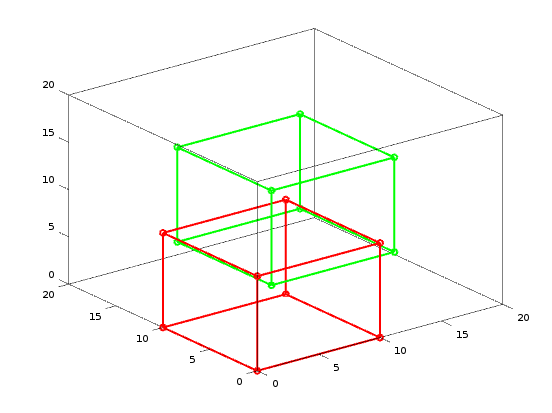
\includegraphics[width=150mm, height=100mm]{translation.png}
\caption{translation \label{overflow}}
\end{figure}
\begin{figure}[ht!]
\centering
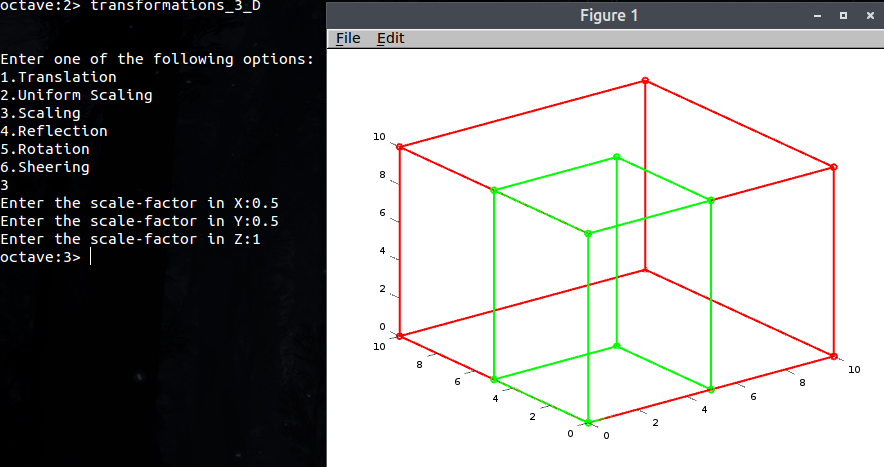
\includegraphics[width=150mm, height=100mm]{scaling.png}
\caption{scaling \label{overflow}}
\end{figure}
\begin{figure}[ht!]
\centering
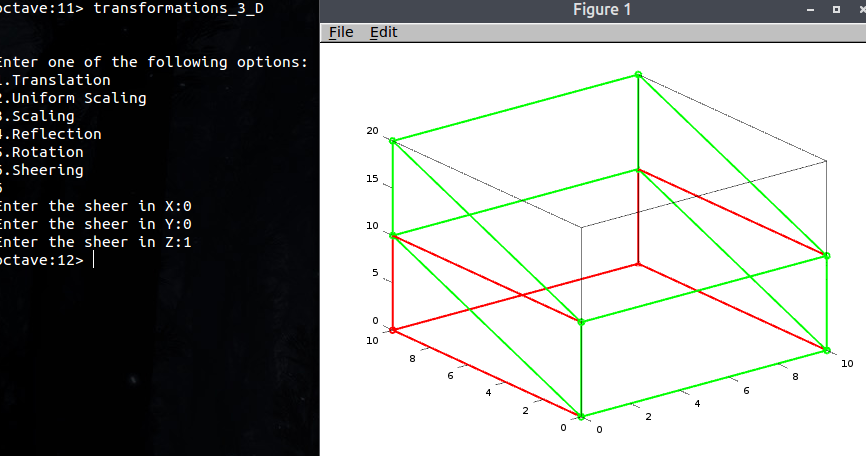
\includegraphics[width=150mm, height=100mm]{sheer.png}
\caption{sheer \label{overflow}}
\end{figure}
\begin{figure}[ht!]
\centering
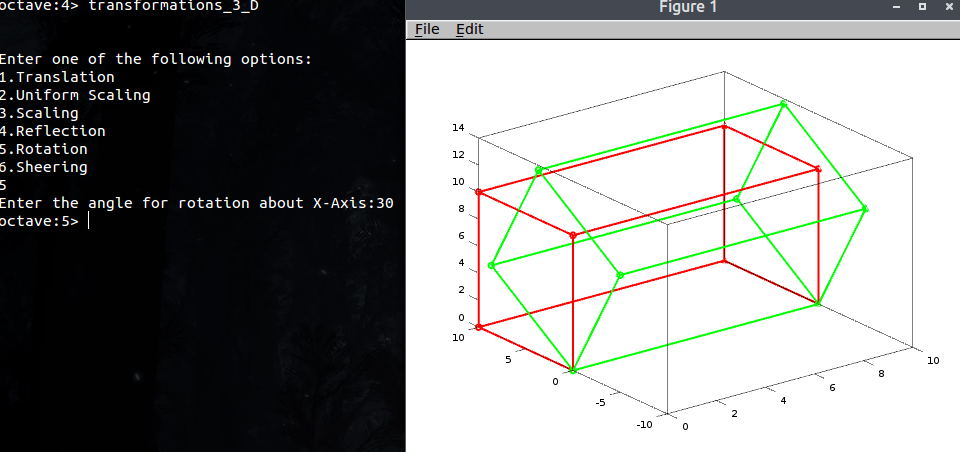
\includegraphics[width=150mm, height=100mm]{rotation.png}
\caption{rotation \label{overflow}}
\end{figure}
\begin{figure}[ht!]
\centering
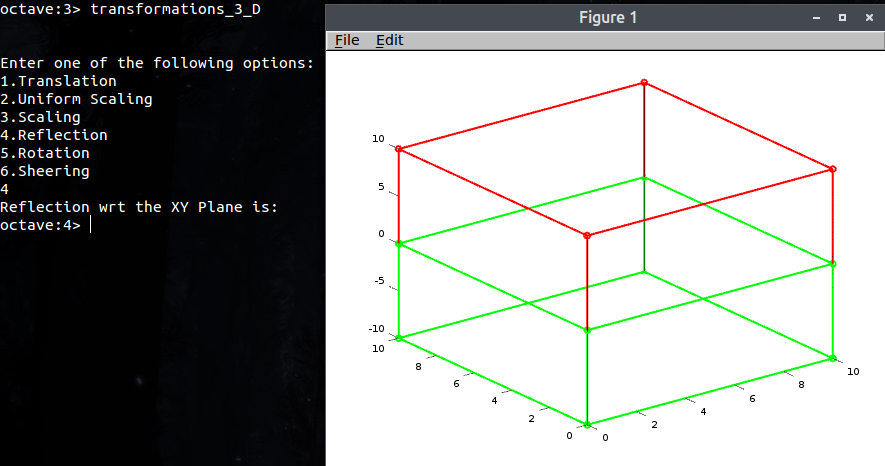
\includegraphics[width=150mm, height=100mm]{reflection.png}
\caption{reflection \label{overflow}}
\end{figure}
\end{document}
